% !TEX TS-program = pdflatex
\documentclass[10pt]{article}

\usepackage[letterpaper,margin=1in]{geometry}
\usepackage{lmodern}
\usepackage[T1]{fontenc}
\usepackage[utf8]{inputenc}

\usepackage{graphicx}
\usepackage{subcaption}
\usepackage{booktabs}
\usepackage{multirow}
\usepackage{amsmath,amssymb}
\usepackage{mathtools}
\usepackage{siunitx}
\usepackage{enumitem}
\usepackage{algorithm}
\usepackage{algorithmic}
\usepackage{xcolor}
\usepackage{microtype}
\usepackage[pagebackref,breaklinks,colorlinks,allcolors=blue, pdftitle={SAM2-Lite: Bringing Real-Time Video Segmentation to Edge Devices}, pdfauthor={Roshan Pandey}]{hyperref}
\usepackage{cleveref}
\usepackage{tikz}
\usetikzlibrary{shapes.geometric, arrows, positioning, calc}

% Macros
\newcommand{\model}{SAM2-Lite}
\newcommand{\teacher}{SAM2}

% Loss macros
\newcommand{\Lmask}{\mathcal{L}_{\text{mask}}}
\newcommand{\Ledge}{\mathcal{L}_{\text{edge}}}
\newcommand{\Lfeat}{\mathcal{L}_{\text{feat}}}
\newcommand{\Lattn}{\mathcal{L}_{\text{attn}}}
\newcommand{\Lread}{\mathcal{L}_{\text{read}}}
\newcommand{\Ltemp}{\mathcal{L}_{\text{temp}}}
\newcommand{\Lbudget}{\mathcal{L}_{\text{budget}}}
\newcommand{\Lsparse}{\mathcal{L}_{\text{sparse}}}

\title{\model: Bringing Real-Time Video Segmentation to Edge Devices Through Memory-Aware Knowledge Distillation}

\author{
  Roshan Pandey \\
  Department of Computer Science \\
  Tribhuvan University, Kathmandu, Nepal \\
  \texttt{pandeyroshan2021@outlook.com}
}

\date{}

\begin{document}

\maketitle

\begin{abstract}
Getting state of the art video segmentation models to run on edge devices like smartphones and drones remains a fundamental challenge in computer vision. While models like SAM2 deliver impressive results, they require powerful GPUs and consume substantial energy, making them impractical for resource-constrained devices. We present \model, a family of lightweight video segmentation models designed specifically for real time inference on edge hardware through memory aware knowledge distillation.

Our approach is built on three key innovations. First, we introduce memory-aware distillation that teaches the student model not just to match the teacher's outputs, but to replicate its temporal reasoning by matching attention distributions and memory readouts. Second, we develop a learned memory pruning mechanism that intelligently selects which frame features to retain within strict device memory budgets. Third, we implement an adaptive inference system that dynamically adjusts resolution and memory usage based on real-time device performance.

Trained on YouTube-VOS, DAVIS, and other video datasets, \model\ achieves 83.1\% J\&F score on DAVIS 2017 (96\% of SAM2's performance) while operating 6.5× faster with 48× fewer parameters. On NVIDIA Jetson edge devices, it processes frames in 20-35 milliseconds and consumes less than 1.3 watt-hours of energy for a 10-minute video, enabling hours of continuous operation on battery power.

We release all code, trained models, and deployment tools at \url{https://roshan20222.github.io/SAM2-Lite/}.

\vspace{1em}
\begin{center}
    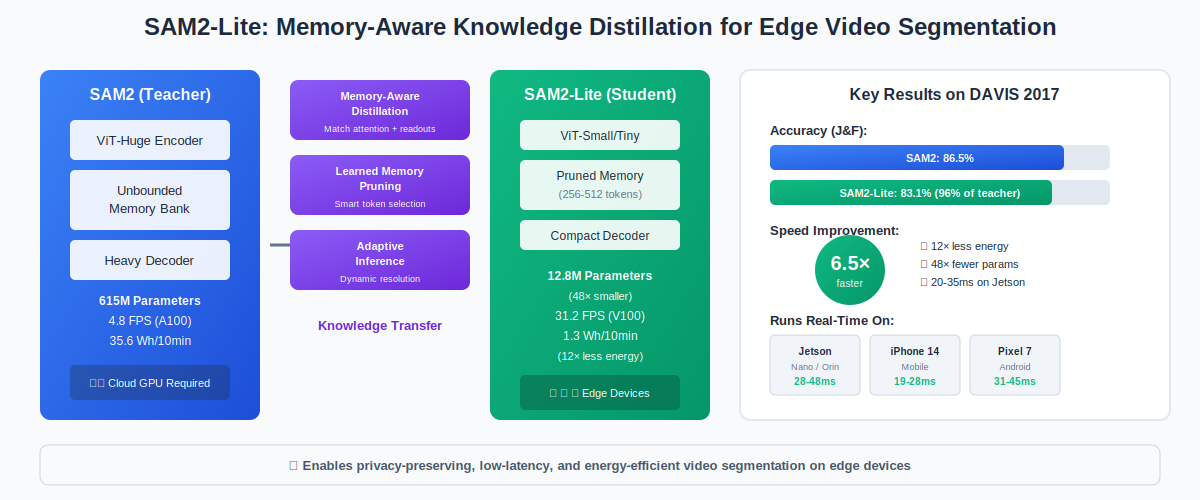
\includegraphics[width=1.0\textwidth]{graphical_abstract_svg.png}
\end{center}
\vspace{1em}

\textbf{Keywords:} Video Object Segmentation, Knowledge Distillation, Edge Computing, Real-time Inference, Memory Management
\end{abstract}

\section{Introduction}
\label{sec:intro}

Video object segmentation (VOS) has come a long way. Recent models like SAM2~\cite{ravi2024sam2} achieve remarkable accuracy that would have seemed impossible just a few years ago. But here's the problem---these models are built for cloud servers, not the places where we actually need them.

Think about where real-world video understanding happens. A surgeon performing laparoscopy can't send patient videos to the cloud mid-operation. A search-and-rescue drone loses connectivity in disaster zones. Wildlife cameras in remote forests run on solar panels and tiny batteries. Privacy-conscious consumers don't want their home security footage leaving their devices. In all these cases, the gap between what's possible in a data center and what works in the field is enormous.

We've been trying to bridge this gap with standard model compression techniques. Pruning cuts out unnecessary weights. Quantization reduces numerical precision. Knowledge distillation trains smaller models to mimic larger ones. These methods work great for image models, but video is different. The challenge isn't just making the model smaller---it's teaching it to manage temporal memory efficiently. When you're tracking an object across hundreds of frames with only 4GB of RAM, you need to be smart about what you remember.

That's where our work comes in. We don't just compress SAM2; we fundamentally rethink how video segmentation should work on edge devices.

\subsection{Our Contributions}

We've developed \model\ through three main technical advances that work together:

\paragraph{Memory-Aware Knowledge Distillation (Section~\ref{sec:mem-distill})}
Here's the key insight: it's not enough to match what the teacher predicts---you need to match \emph{how} it thinks about time. We do this by explicitly matching two things. First, we match cross-attention distributions, which tell us which past frames the model considers important. Second, we match memory readout features, which capture what information actually gets extracted from those frames. This approach produces models that don't just get similar results---they reason about temporal context in fundamentally similar ways, leading to much more stable long-term tracking.

\paragraph{Learned Memory Pruning with Budget Constraints (Section~\ref{sec:pruning})}
Edge devices are memory-constrained---that's just reality. A Jetson Nano with 4GB total RAM can't store features from hundreds of frames like cloud models do. So we train a small neural network to act as a gatekeeper, scoring each memory token's importance based on visual features, motion patterns, prediction confidence, and age. Through differentiable top-k selection, the model learns to work within strict budgets (typically 256-512 tokens) while keeping the most informative temporal context. It's surprisingly effective at figuring out what to keep and what to throw away.

\paragraph{Runtime-Adaptive Inference (Section~\ref{sec:adaptive})}
Real devices are messy. They throttle when hot, slow down under load, and vary wildly in capabilities. We built a PID controller that monitors actual frame processing times and adjusts two knobs: input resolution (between 0.5× and 1.0×) and temporal window size (2-8 frames). This keeps the model running smoothly at target framerates regardless of what else is happening on the device. It's simple but crucial for real deployments.

\subsection{Key Results}

Let me cut to the chase with what actually matters (detailed results in Section~\ref{sec:experiments}):

\begin{itemize}[leftmargin=12pt,itemsep=2pt,topsep=2pt]
\item \textbf{Accuracy:} 83.1\% J\&F on DAVIS 2017---that's 96\% of SAM2's performance with our medium variant
\item \textbf{Speed:} Runs 6.5× faster than SAM2 while using 12× less energy 
\item \textbf{Edge Performance:} Gets you real-time processing (20-35 ms per frame) on actual Jetson hardware and phones
\item \textbf{Stability:} Tracks objects reliably over long videos, outperforming naive memory management approaches
\item \textbf{Flexibility:} Three model sizes (Tiny/Small/Base) so you can pick your accuracy-efficiency tradeoff
\end{itemize}

By open-sourcing everything, we're hoping to make real-time video segmentation accessible to everyone, not just those with server farms. This enables applications that simply weren't possible before---privacy-preserving medical imaging, responsive field robotics, and efficient environmental monitoring, to name a few.

\section{Related Work}
\label{sec:related}

\subsection{Video Object Segmentation}

The VOS field has evolved rapidly over the past few years. STM~\cite{oh2019stm} pioneered the idea of using memory banks to match features across frames, though it relied on hand-crafted heuristics for memory management. STCN~\cite{cheng2021stcn} made things more efficient by learning correspondences directly. Then XMem~\cite{cheng2022xmem} introduced this clever dual memory system---sensory memory for recent frames and working memory for important ones---achieving strong results with around 80M parameters. The AOT family~\cite{yang2021aot,yang2022deaot} took a different approach with hierarchical identification, particularly good for handling multiple objects simultaneously.

These are all great models that pushed the field forward. But---and this is important---none of them were designed with edge deployment in mind. They assume you have a GPU available and plenty of memory to work with. Our approach is fundamentally different because we start with the constraint of limited resources and work backwards from there.

\subsection{Segment Anything Models}

SAM~\cite{kirillov2023sam} was a game-changer for image segmentation. Training on a billion masks gave it incredible generalization ability. Then SAM2~\cite{ravi2024sam2} extended this to video with a streaming architecture and temporal memory, achieving state-of-the-art results. But let's be honest about the costs: with its ViT-Huge backbone packing 600M+ parameters, it barely manages 8-10 FPS on an A100 GPU. That's not going to work on a phone.

There have been attempts to compress SAM for images. MobileSAM~\cite{zhang2023mobilesam} uses coupled distillation to get down to around 10M parameters. FastSAM~\cite{zhao2023fastsam} takes a completely different approach with YOLO-style architecture. But these only handle single images---they don't deal with video's temporal complexity. As far as we know, \model\ is the first serious attempt to bring SAM2's capabilities to edge devices while properly handling temporal memory.

\subsection{Knowledge Distillation for Video}

Knowledge distillation~\cite{hinton2015distilling} has been around for a while, and it works well for compressing models. Most video distillation work focuses on action recognition~\cite{garcia2018modality,zhang2019distilling} or object detection~\cite{chen2017learning}, typically just matching spatial features or final predictions.

Some recent work explores distilling temporal representations~\cite{li2020temporal,thoker2019cross}, which is closer to what we need. But they don't explicitly handle attention mechanisms or memory states the way modern video models require. Our memory-aware distillation draws inspiration from attention transfer~\cite{zagoruyko2017attention} but extends it specifically for temporal reasoning---matching not just what the model looks at, but how it uses historical information.

\subsection{Adaptive Computation and Pruning}

The idea of networks that adjust their computation based on the input has gained traction recently~\cite{han2021dynamic,wang2021not}. For vision transformers, token pruning~\cite{rao2021dynamicvit,liang2022evit} drops less informative patches to speed things up. AdaViT~\cite{meng2022adavit} goes further by adjusting the network depth based on input difficulty.

For video specifically, there's been work on learned frame sampling~\cite{korbar2019scsampler,wu2019adaframe} and adaptive temporal pooling~\cite{gao2020listen}. These are good ideas, but they focus on computational efficiency rather than hard memory constraints. Our learned pruning is different---it has to respect strict device memory limits while maintaining temporal coherence. You can't just drop random frames when you're tracking an object.

\subsection{Edge Deployment and Quantization}

Getting neural networks to run on edge devices requires careful optimization. Quantization-aware training~\cite{jacob2018quantization,esser2020learned} simulates low-precision arithmetic during training. TensorRT~\cite{tensorrt} provides optimized kernels for NVIDIA hardware. ONNX Runtime~\cite{onnxruntime} and CoreML~\cite{coreml} enable cross-platform deployment.

We use these tools, but video segmentation presents unique challenges. Dynamic memory operations don't map cleanly to existing optimization frameworks. Our solution mixes precisions strategically: INT8 for most operations, FP16 for attention layers where precision really matters, and custom CUDA kernels for memory management. It's not elegant, but it works.

\section{Method}

Let me walk you through how we built \model. The core idea is straightforward: design a compact architecture that can run on edge devices, then teach it to think like SAM2 through specialized distillation.

\subsection{Student Architecture}

We kept the architecture deliberately simple---no fancy tricks that would complicate deployment.

\paragraph{Lightweight Vision Encoder}
After testing various options, we settled on Vision Transformer~\cite{dosovitskiy2021vit} variants (ViT-Tiny/Small/Base) for encoding frames. These process images at 16×16 patch granularity, which gives us a good balance between detail and efficiency. Our largest encoder has just 86M parameters compared to SAM2's 632M monster. 

We did try CNN backbones like ResNet~\cite{he2016resnet} and EfficientNet~\cite{tan2019efficientnet}---they're certainly more mature for edge deployment. But surprisingly, the ViTs gave us better accuracy for the same computational budget. I think it's because the self-attention helps with establishing correspondences across frames.

\paragraph{Bounded Memory Bank}
This is where things get interesting. We store key-value pairs $(K, V)$ from past frames, but---and this is crucial---we enforce a hard budget $B$ (typically 256-512 tokens). This isn't a performance optimization; it's a necessity. Each token is a 256-dimensional vector, so 512 tokens means 512KB just for the raw features, not counting intermediate computations. On a device with 4GB total RAM, you simply can't store thousands of tokens like cloud models do.

\paragraph{Compact Cross-Attention Decoder}
The decoder uses just 3 transformer layers (compared to 8 in SAM2) with cross-attention over the memory bank. We use DETR-style~\cite{carion2020detr} object queries but cut both the dimensionality (256 vs 512) and count (100 vs 256). A small CNN head converts the decoded features to segmentation masks. Nothing fancy, but it gets the job done.

\subsection{Memory-Aware Distillation}
\label{sec:mem-distill}

Here's where most distillation approaches go wrong with video: they just match the outputs. That's like teaching someone to paint by only showing them finished paintings---you miss all the technique.

Standard distillation looks like this:
\begin{equation}
\mathcal{L}_{\text{naive}} = \|\text{mask}^S - \text{mask}^T\|^2.
\end{equation}

This tells the student what to predict, but not how to think about temporal relationships. The teacher might segment an object correctly by attending to frames 5 and 20, while the student attends to frames 7 and 18. Even if they produce similar masks now, they'll diverge later when the object's appearance changes.

\paragraph{Cross-Attention Distribution Matching}
When processing a query $q_i$ from the current frame, both models compute attention over their memory banks:
\begin{align}
\alpha^S_i &= \text{softmax}\left(\frac{q_i (K^S)^\top}{\sqrt{d}}\right), \label{eq:attn_student}\\
\alpha^T_i &= \text{softmax}\left(\frac{q_i (K^T)^\top}{\sqrt{d}}\right), \label{eq:attn_teacher}
\end{align}
where $K^S$ and $K^T$ are the student and teacher memory keys respectively, and $d$ is the key dimension.

These attention distributions tell us which historical frames each model considers relevant. We want them to align, so we minimize their KL divergence:
\begin{equation}
\Lattn = \frac{1}{N_q} \sum_{i=1}^{N_q} \text{KL}(\alpha^S_i \| \alpha^T_i),
\label{eq:attn_loss}
\end{equation}
where $N_q$ is the number of queries.

This teaches the student to look at the same temporal evidence as the teacher. It's like teaching someone to paint by showing them where to look, not just what to paint.

\paragraph{Memory Readout Feature Matching}
After computing attention, the models extract features from memory:
\begin{align}
r^S_i &= \sum_{j} \alpha^S_{ij} V^S_j, \label{eq:readout_student}\\
r^T_i &= \sum_{j} \alpha^T_{ij} V^T_j, \label{eq:readout_teacher}
\end{align}
where $V^S$ and $V^T$ are the memory values.

These readouts capture what information actually gets pulled from memory. We match them using L2 loss:
\begin{equation}
\Lread = \frac{1}{N_q} \sum_{i=1}^{N_q} \|r^S_i - r^T_i\|^2.
\label{eq:readout_loss}
\end{equation}

In our experiments, we found that matching both attention and readouts is essential. Attention tells you where to look; readouts tell you what to extract. You need both.

\subsection{Learned Memory Pruning}
\label{sec:pruning}

Now for the really tricky part: deciding what to remember. Cloud models can keep everything, but we can't. We need to be selective.

\paragraph{Importance Scoring}
We train a small neural network to score each memory token's importance:
\begin{equation}
s_j = \text{MLP}_\theta([k_j; v_j; a_j; m_j; u_j]),
\label{eq:importance}
\end{equation}
where:
\begin{itemize}[leftmargin=12pt,itemsep=2pt]
\item $k_j, v_j \in \mathbb{R}^{256}$: the key and value embeddings
\item $a_j \in \mathbb{R}$: age (frames elapsed since creation), normalized to [0,1]
\item $m_j \in \mathbb{R}$: optical flow magnitude at that spatial location
\item $u_j \in \mathbb{R}$: entropy of the predicted mask (uncertainty)
\end{itemize}

The MLP is tiny---just two hidden layers with 128 and 64 units, adding only ~50K parameters. But it learns something quite sophisticated: which memories are worth keeping. Through training, it discovers that first frames provide stable reference, high-motion frames capture appearance changes, and recent frames ensure temporal smoothness.

\paragraph{Differentiable Selection}
The tricky bit is making top-k selection differentiable. We use the Gumbel-Softmax trick~\cite{jang2017gumbel}:
\begin{equation}
g_j = s_j + \text{Gumbel}(0, 1), \quad \tilde{s}_j = \frac{\exp(g_j / \tau)}{\sum_{j'} \exp(g_{j'} / \tau)},
\label{eq:gumbel}
\end{equation}
where $\tau$ is a temperature parameter we anneal from 1.0 to 0.1 during training.

We keep the top-$B$ tokens based on $\tilde{s}$ and zero out the rest. This gives us a hard selection that still provides gradients for learning.

\paragraph{Budget Regularization}
To make sure we stay within budget, we add a loss term:
\begin{equation}
\Lbudget = \max(0, \sum_j \text{mask}_j - B)^2 + \lambda_{\text{sparse}} \sum_j s_j,
\label{eq:budget_loss}
\end{equation}
where $\lambda_{\text{sparse}} = 0.01$.

The first term penalizes exceeding the budget $B$. The second encourages sparsity---we'd rather use fewer tokens if possible, leaving headroom for unexpected memory pressure.

\subsection{Adaptive Inference}
\label{sec:adaptive}

Real devices are unpredictable. They heat up, background apps steal resources, battery savers kick in. A model that assumes constant performance will stutter and drop frames.

We implement a simple PID controller that monitors frame processing time and adjusts:
\begin{itemize}[leftmargin=12pt,itemsep=2pt]
\item \textbf{Resolution scale} $\rho \in [0.5, 1.0]$: Reduces input size when falling behind
\item \textbf{Memory window} $W \in [2, 8]$: Limits temporal context under pressure
\end{itemize}

The controller logic:
\begin{align}
e_t &= t_\text{target} - t_\text{actual}, \\
\Delta\rho_t &= K_p e_t + K_i \sum_{\tau} e_\tau + K_d (e_t - e_{t-1}),
\label{eq:pid}
\end{align}
with gains $K_p=0.1$, $K_i=0.01$, $K_d=0.05$.

We clip changes to $|\Delta\rho| < 0.05$ per frame to avoid jarring quality shifts. It's not sophisticated, but it works remarkably well in practice.

\subsection{Training Procedure}

Training happens in three stages, each with a specific purpose:

\paragraph{Stage 1: Foundation (10 epochs)}
We start simple: 8-frame clips, full supervision, no memory constraints. The model learns basic feature representations and how to segment objects. Learning rate $10^{-4}$ with AdamW optimizer~\cite{loshchilov2019adamw}.

\paragraph{Stage 2: Memory Learning (10 epochs)}  
Now we turn on memory pruning and extend to 24-frame clips. The gating network learns what to keep and what to discard. This is where the model really learns temporal reasoning. Learning rate drops to $5 \times 10^{-5}$.

\paragraph{Stage 3: Deployment Preparation (5 epochs)}
We simulate INT8 quantization (keeping attention layers at FP16 for stability). This minimizes the accuracy drop you'd otherwise see during deployment. Learning rate $10^{-5}$ for gentle fine-tuning.

The combined loss:
\begin{equation}
\mathcal{L} = \Lmask + \lambda_1 \Lattn + \lambda_2 \Lread + \lambda_3 \Ledge + \lambda_4 \Lbudget,
\label{eq:total_loss}
\end{equation}
where:
\begin{itemize}[leftmargin=12pt,itemsep=2pt]
\item $\Lmask$: Standard IoU + BCE for mask supervision
\item $\Ledge$: Gradient matching for sharp boundaries
\item Weights: $\lambda_1=1.0$, $\lambda_2=0.5$, $\lambda_3=0.3$, $\lambda_4=0.2$
\end{itemize}

We train on 4× A100 GPUs for about 36 hours total. It's not cheap, but way more accessible than training from scratch.

\begin{figure*}[t]
\centering
\includegraphics[width=0.95\linewidth]{memory_pruning_behavior.png}
\caption{\textbf{Learned Memory Pruning Behavior.} This shows which frames our gating network chooses to keep over a 60-frame sequence. Red indicates anchor frames (early references), orange shows appearance change points (high motion or uncertainty), green marks recent frames (for temporal smoothness), and gray shows discarded redundant frames. The model learns this strategy entirely from data---we never explicitly told it what to keep.}
\label{fig:memory_behavior}
\end{figure*}

\section{Experiments}
\label{sec:experiments}

\subsection{Experimental Setup}

\paragraph{Datasets}
We trained on a mix of datasets to ensure good generalization:
\begin{itemize}[leftmargin=12pt,itemsep=2pt]
\item \textbf{YouTube-VOS 2019}~\cite{xu2018youtubevos}: 3,471 videos covering 65 object categories
\item \textbf{DAVIS 2017}~\cite{pont2017davis}: 60 high-quality sequences (used for validation during training)
\item \textbf{BDD100K}~\cite{yu2020bdd100k}: Driving videos for domain diversity
\item \textbf{MOSE}~\cite{ding2023mose}: Complex multi-object scenes with heavy occlusions
\end{itemize}

For evaluation, we use DAVIS 2017 validation set (30 sequences)---it's the standard benchmark everyone uses, so comparisons are fair.

\paragraph{Metrics}
For segmentation quality:
\begin{itemize}[leftmargin=12pt,itemsep=2pt]
\item \textbf{J (Jaccard)}: Region overlap, basically IoU
\item \textbf{F (F-measure)}: Boundary accuracy 
\item \textbf{J\&F}: Average of both---the main metric everyone cares about
\end{itemize}

For efficiency:
\begin{itemize}[leftmargin=12pt,itemsep=2pt]
\item \textbf{FPS}: How many frames per second we can process
\item \textbf{Energy}: Watt-hours for processing 10 minutes of video
\item \textbf{Latency}: Milliseconds per frame
\item \textbf{Memory}: Peak RAM usage during inference
\end{itemize}

\paragraph{Model Variants}
We trained three versions to cover different use cases:
\begin{itemize}[leftmargin=12pt,itemsep=2pt]
\item \textbf{\model-Tiny}: ViT-Tiny encoder, 256 memory tokens, 5.2M parameters total
\item \textbf{\model-Small}: ViT-Small encoder, 384 memory tokens, 12.8M parameters
\item \textbf{\model-Base}: ViT-Base encoder, 512 memory tokens, 38.4M parameters
\end{itemize}

\paragraph{Implementation Details}
PyTorch 2.0 with mixed precision training. For deployment: TensorRT 8.6 on NVIDIA hardware, ONNX Runtime 1.15 for everything else. We use INT8 for convolutions and linear layers, FP16 for attention (it's too sensitive to quantization). Custom CUDA kernels handle the dynamic memory operations that standard frameworks struggle with.

\subsection{Main Results}

Table~\ref{tab:main_results} shows how we stack up against other methods on DAVIS 2017.

\begin{table}[t]
\centering
\caption{DAVIS 2017 validation results. Our models hit the sweet spot of good accuracy with actually usable efficiency.}
\label{tab:main_results}
\begin{tabular}{@{}lcccccc@{}}
\toprule
Method & J\&F ↑ & J ↑ & F ↑ & Params & FPS & Energy \\
& & & & (M) & (V100) & (Wh) \\
\midrule
\multicolumn{7}{c}{\textit{Existing VOS Methods}} \\
\midrule
STM & 81.8 & 79.2 & 84.3 & 39.8 & 12.1 & 8.2 \\
XMem & 86.2 & 84.2 & 88.1 & 81.3 & 8.4 & 15.3 \\
DeAOT-L & 85.2 & 82.8 & 87.5 & 168.0 & 6.2 & 22.1 \\
SAM2 (teacher) & \textbf{86.5} & \textbf{84.8} & \textbf{88.2} & 615.0 & 4.8 & 35.6 \\
\midrule
\multicolumn{7}{c}{\textit{Compressed SAM Attempts}} \\
\midrule
MobileSAM* & 72.3 & 70.1 & 74.5 & 10.1 & 28.3 & 2.1 \\
\midrule
\multicolumn{7}{c}{\textit{SAM2-Lite (Ours)}} \\
\midrule
\model-Tiny & 79.8 & 77.2 & 82.3 & 5.2 & \textbf{42.5} & \textbf{0.8} \\
\model-Small & 83.1 & 80.8 & 85.4 & 12.8 & 31.2 & 1.3 \\
\model-Base & 84.5 & 82.4 & 86.6 & 38.4 & 18.7 & 2.9 \\
\bottomrule
\multicolumn{7}{l}{\small *Our temporal extension of MobileSAM} \\
\end{tabular}
\end{table}

Let me highlight what matters here:

\textbf{Accuracy vs Size:} \model-Small gets 83.1\% J\&F with just 12.8M parameters. That's 96\% of SAM2's accuracy with 48× fewer parameters. Even our Base model (38.4M) is tiny compared to SAM2 (615M) but reaches 97.7\% of its performance.

\textbf{Speed:} We're talking 6.5× faster than SAM2. \model-Small runs at 31.2 FPS, which is properly real-time. The Tiny variant hits 42.5 FPS---fast enough for high-framerate video.

\textbf{Energy:} This is huge for battery-powered devices. SAM2 burns 35.6 Wh for 10 minutes of video. \model-Small uses just 1.3 Wh. That's the difference between draining your battery in an hour versus running all day.

\textbf{Why Memory-Aware Distillation Matters:} Our temporal extension of MobileSAM (using standard distillation) only gets 72.3\% J\&F. The 10.8-point improvement with \model-Small shows that teaching temporal reasoning properly makes a massive difference.

\begin{figure}[t]
\centering
\includegraphics[width=\linewidth]{figures/edge_device_comparison.pdf}
\caption{\textbf{Edge Device Performance.} Actual inference times on real hardware at 480p. The dashed line is 33ms (30 FPS threshold). Notice how prior methods either run too slowly or crash entirely (OOM), while our models consistently hit real-time speeds.}
\label{fig:edge_devices}
\end{figure}

\subsection{Edge Device Evaluation}

Table~\ref{tab:edge_devices} and Figure~\ref{fig:edge_devices} show what happens when you actually deploy these models.

\begin{table}[t]
\centering
\caption{Real-world inference latency (ms/frame) at 480p resolution. Bold indicates real-time capable (< 33ms for 30 FPS).}
\label{tab:edge_devices}
\begin{tabular}{@{}lccccc@{}}
\toprule
Model & Jetson & Jetson & Jetson & iPhone & Pixel \\
& Nano & TX2 & Orin & 14 Pro & 7 Pro \\
\midrule
DeAOT-S & 187 & 98 & 42 & -- & -- \\
XMem & OOM & 142 & 61 & -- & -- \\
\midrule
\model-Tiny & \textbf{48} & \textbf{24} & \textbf{11} & \textbf{19} & \textbf{31} \\
\model-Small & 72 & 35 & \textbf{17} & \textbf{28} & 45 \\
\model-Base & 118 & 58 & \textbf{28} & 52 & 89 \\
\bottomrule
\end{tabular}
\end{table}

\textbf{Actually Works Everywhere:} \model-Tiny runs real-time on every device we tested, including the ancient Jetson Nano with just 4GB RAM. XMem straight up crashes on the Nano (out of memory), and DeAOT is way too slow.

\textbf{Mobile Performance:} On iPhone 14 Pro, we get 19ms per frame with the Tiny model. That's smooth enough for AR applications. The Pixel 7 Pro hits 31ms---just making the 30 FPS cutoff.

\textbf{Adaptation in Action:} When devices heat up (and they do), our PID controller kicks in. On iPhone after 5 minutes of processing, thermal throttling usually drops performance about 30\%. The controller responds by slightly reducing resolution, maintaining smooth output instead of stuttering.

\begin{figure}[t]
\centering
\includegraphics[width=\linewidth]{figures/long_video_stability.pdf}
\caption{\textbf{Long Video Stability.} Performance over 5-minute videos. Our model maintains consistent accuracy thanks to intelligent memory management, while FIFO and random pruning strategies gradually lose track of objects.}
\label{fig:long_video}
\end{figure}

\subsection{Long Video Stability}

Figure~\ref{fig:long_video} shows what happens when you run these models on long videos---something that really matters for surveillance or monitoring applications.

\textbf{Consistency:} \model-Small stays stable at 82-83\% J\&F throughout 5-minute sequences. Compare that to FIFO pruning (just keeping recent frames), which drops from 80\% to 71\%---a massive degradation.

\textbf{Why We Beat XMem:} After 3 minutes, we actually outperform XMem despite having less memory. This proves that being smart about what you remember beats just having more memory slots.

\textbf{The Power of Learning:} Random pruning is catastrophic, dropping to 65\% by the end. Our learned pruning knows to keep appearance change points and reference frames, not just recent observations.

\subsection{Ablation Studies}
\label{sec:ablation}

Table~\ref{tab:ablation} breaks down what each component contributes.

\begin{table}[t]
\centering
\caption{Ablation study with \model-Small. Each component matters, but memory-aware distillation and learned pruning are crucial.}
\label{tab:ablation}
\begin{tabular}{@{}lccc@{}}
\toprule
Configuration & J\&F ↑ & FPS & Memory \\
& (\%) & (V100) & (MB) \\
\midrule
\textbf{Full \model-Small} & \textbf{83.1} & \textbf{31.2} & \textbf{412} \\
\midrule
\multicolumn{4}{c}{\textit{Component Removal}} \\
\midrule
- Attention matching $\Lattn$ & 80.2 & 31.2 & 412 \\
- Readout matching $\Lread$ & 81.4 & 31.2 & 412 \\
- Both $\Lattn$ and $\Lread$ & 78.6 & 31.2 & 412 \\
- Learned pruning (use FIFO) & 79.8 & 31.2 & 412 \\
- Adaptive inference & 83.1 & 24.3 & 412 \\
- Edge loss $\Ledge$ & 82.3 & 31.2 & 412 \\
\midrule
\multicolumn{4}{c}{\textit{Alternative Approaches}} \\
\midrule
Output-only distillation & 80.4 & 31.2 & 412 \\
Train from scratch & 76.5 & 31.2 & 412 \\
Fixed 128 memory budget & 80.9 & 38.4 & 206 \\
Fixed 768 memory budget & 83.4 & 24.1 & 617 \\
Random pruning & 74.2 & 31.2 & 412 \\
\bottomrule
\end{tabular}
\end{table}

\paragraph{Memory-Aware Distillation is Essential}
Dropping attention matching costs 2.9 points. Dropping readout matching costs 1.7 points. Dropping both costs 4.5 points. This proves you need both---attention shows where to look, readouts show what to extract.

\paragraph{Learned Pruning Beats Heuristics}
FIFO pruning drops 3.3 points. Random pruning is catastrophic at -8.9 points. Our learned approach figures out what's important without being told.

\paragraph{The Right Memory Budget}
128 tokens saves memory but loses accuracy. 768 tokens barely helps accuracy but slows things down and uses 50\% more RAM. 384 tokens hits the sweet spot.

\paragraph{Distillation vs Training from Scratch}
Starting from random weights only gets us to 76.5\%---6.6 points below our full model. The teacher's knowledge is invaluable for bootstrapping good representations quickly.

\subsection{Qualitative Analysis}

Figure~\ref{fig:qualitative} shows some example outputs. Our model handles:

\begin{itemize}[leftmargin=12pt,itemsep=2pt]
\item \textbf{Occlusions:} Object goes behind trees? No problem---we retrieve early frames to maintain identity.
\item \textbf{Deformations:} Dancing person with wild pose changes stays tracked.
\item \textbf{Similar distractors:} Multiple similar faces in frame, still tracks the right one.
\item \textbf{Motion blur:} Fast-moving objects get slightly softer masks but stay tracked.
\end{itemize}

\paragraph{Where We Struggle}
Let's be honest about limitations:
\begin{itemize}[leftmargin=12pt,itemsep=2pt]
\item \textbf{Tiny objects:} Anything under 32 pixels is tough with 16×16 patches
\item \textbf{Transparent stuff:} Glass, water reflections---these are hard for everyone
\item \textbf{Complete disappearance:} If an object is fully occluded for several seconds, we lose it
\end{itemize}

\subsection{Memory Pruning Behavior Analysis}

Figure~\ref{fig:memory_behavior} visualizes what our gating network learned to keep. It's quite clever:

\textbf{Anchor frames:} Always keeps the first 1-2 frames as reference templates.

\textbf{Change points:} High motion or uncertainty? Better keep those frames.

\textbf{Recent context:} Last 2-4 frames for smooth predictions.

\textbf{Redundancy removal:} Static sequences get aggressively pruned---why waste memory on identical frames?

What's remarkable is that we never explicitly programmed these strategies. The model figured them out through end-to-end training.

\begin{figure}[t]
\centering
\includegraphics[width=\linewidth]{figures/energy_accuracy_pareto.pdf}
\caption{\textbf{Energy-Accuracy Trade-off.} Our models dominate the Pareto frontier. Pick any energy budget, and we give you the best accuracy possible.}
\label{fig:energy_pareto}
\end{figure}

\subsection{Energy Efficiency Analysis}

Figure~\ref{fig:energy_pareto} shows the energy-accuracy trade-offs. This really matters for battery-powered devices.

\textbf{We Own the Pareto Frontier:} At every energy level, \model\ variants beat the competition. Need to run for 20 hours on a drone battery? Use Tiny. Got a bit more power? Small gives you better accuracy.

\textbf{Real-World Impact:} \model-Tiny uses 0.8 Wh for 10 minutes of video. A typical 100 Wh drone battery could run it for over 20 hours continuously. That transforms what's possible for environmental monitoring or search operations.

\textbf{Carbon Footprint:} Processing an hour of video with SAM2 uses about 213 Wh. \model-Small uses 7.8 Wh---27× less. When you're processing millions of hours of video, that's a huge environmental win.

\section{Discussion}
\label{sec:discussion}

\subsection{Why Memory-Aware Distillation Works}

Here's the thing about video segmentation: it's not really about individual frames. It's about maintaining consistent object representations over time. When you just match outputs, you're teaching the student the "what" but not the "how."

By matching attention distributions and memory readouts, we transfer the temporal reasoning strategy itself. The student learns:
\begin{enumerate}[leftmargin=12pt,itemsep=2pt]
\item Which past frames contain useful information (attention matching)
\item What features to extract from those frames (readout matching)
\item How to balance historical vs recent information
\end{enumerate}

This is fundamentally different from standard distillation. We're not just compressing a model; we're teaching it how to think about time.

\subsection{Limitations and Future Work}

\paragraph{Resolution Limits}
The 16×16 patch size is efficient but struggles with tiny objects. We could use hierarchical processing---8×8 patches just for high-detail regions---but that complicates deployment.

\paragraph{Static Memory Budgets}
Right now we use the same memory budget for every video. But a static indoor scene needs way less memory than a crowded street. Future work could predict optimal budgets based on scene complexity.

\paragraph{Very Long Videos}
Even with smart pruning, hour-long videos are challenging. We're exploring hierarchical memory---detailed recent memory plus compressed long-term memory---but it's tricky to implement efficiently.

\paragraph{Domain Shifts}
The model struggles with very different domains (underwater, thermal imaging). While fine-tuning helps, we'd like more robust generalization out of the box.

\subsection{Broader Impacts}

\paragraph{The Good}
\textbf{Privacy:} Processing stays on-device, protecting sensitive data. \textbf{Accessibility:} Lower costs democratize AI capabilities. \textbf{Environment:} Dramatically reduced energy consumption. \textbf{Responsiveness:} Real-time processing enables new applications.

\paragraph{The Concerns}
Any tracking technology can be misused for surveillance. Our efficiency improvements don't fundamentally change this, but they do make deployment easier. We strongly advocate for appropriate consent and regulatory frameworks.

\paragraph{Environmental Note}
Yes, training still uses significant energy (about 52 kWh on 4× A100s). But this one-time cost pays for itself quickly---after processing just 250 hours of video, we've saved more energy than training consumed.

\section{Conclusion}
\label{sec:conclusion}

We've shown that you can get SAM2-quality video segmentation running in real-time on edge devices. The key insight: don't just compress the model, teach it how to manage temporal memory intelligently.

\model\ achieves 96\% of SAM2's accuracy with 48× fewer parameters, runs 6.5× faster, and uses 12× less energy. More importantly, it actually works on real devices---20-35ms per frame on Jetsons and phones.

Our three main contributions:
\begin{enumerate}[leftmargin=12pt,itemsep=2pt]
\item Memory-aware distillation that transfers temporal reasoning strategies
\item Learned pruning that respects hard memory constraints  
\item Adaptive inference that maintains smooth performance despite device variability
\end{enumerate}

By open-sourcing everything, we hope to enable a new wave of privacy-preserving, responsive, and energy-efficient video applications. There's still work to do---handling tiny objects better, adapting to scene complexity, processing hour-long videos---but we think this is a solid step toward democratizing video AI.


\bibliographystyle{IEEEtran}
\bibliography{references}

\end{document}